\documentclass{article}

\usepackage{tikz}
\usetikzlibrary{snakes,arrows,shapes}
\title{Transition-based parsing of word lattices}
\author{Benoit Favre (benoit.favre@lif.univ-mrs.fr}
\date{\today}

\begin{document}
\maketitle

\section{Introduction}

This document describes a transition-based parser for word lattices. It produces one parse tree for each path of the input using a greedy
algorithm that selects the best action to perform given a context. The resulting forest is provided in a compact action-lattice representation.

\section{Data structures}

\begin{itemize}
\item The {\it input} is a lattice of (word, pos-tag) couples. It is stored as a set of states and each state defines a list of outgoing arcs that include a word/tag label and a state id. The lattice is a directed acyclic graph.
\item The {\it stack} is a tree structure that represents the shared state of the stacks used for transition parsing. Each stack can be seen as a linked list of parse tree nodes. Each node points to a set of children nodes in the parse tree and to a next node in the stack.
\item The list of {\it open} parses contains contexts representing partial parses (stack ending node, next input state, context filter).
\item A {\it context} is the information necessary for extracting features at a given location in the input. If the input is non ambiguous regarding this information (arcs yield the context info), it is just an arc pointer. Otherwise, it's a list of arc pointers necessary for recovering the context (generally the next 3 words).
\end{itemize}

\section{Algorithm}

Initialization:
\begin{itemize}
\item Enumerate starting contexts and push them to the list of open parses with empty stacks.
\end{itemize}

Loop until list of open parses is empty:
\begin{itemize}
\item For each context in list of open parses
    \begin{itemize}
    \item Extract features
    \item Choose action from shift, left arc and right arc
    \item If final state and stack has a single element, add it to the output
    \item Perform action (described in the following sections)
    \item Add new contexts from input to open parses
    \end{itemize}
\end{itemize}

\section{Extending a context}

If the input lattice is non-context-ambiguous, extending a context corresponds to listing the outgoing arcs of the next state.
Otherwise, it corresponds to listing the outgoing arcs of the state next to the furthest word in the context.

\section{Shift (context)}

Preconditions: final state not reached

Given a stack ending in $S_0$, push the next input token in the stack. Extend the context and add the new contexts to the list of open parses.
%We assume that the input graph is contextualized so that feature extraction is not ambiguous.

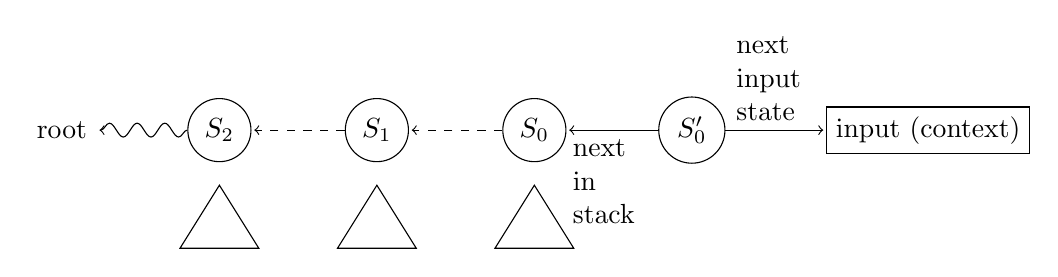
\begin{tikzpicture}[shorten >=1pt,->]
\node at (0,0) (root) {root};
\node[circle,draw] at (2,0) (c) {$S_2$};
\node[circle,draw] at (4,0) (b) {$S_1$};
\node[circle,draw] at (6,0) (top) {$S_0$};
\node[circle,draw] at (8,0) (new) {$S_0'$};
\node[draw] at (11,0) (input) {input (context)};
\draw[snake=snake] (c) -- (root);
\draw[dashed] (top) -- (b);
\draw[dashed] (b) -- (c);
\draw[sharp corners] (6,-0.7) -- (6.5,-1.5) -- (5.5,-1.5) -- cycle;
\draw[sharp corners] (4,-0.7) -- (4.5,-1.5) -- (3.5,-1.5) -- cycle;
\draw[sharp corners] (2,-0.7) -- (2.5,-1.5) -- (1.5,-1.5) -- cycle;
\draw (new) -- node [anchor=north] {\parbox{1cm}{next in stack}} (top);
\draw (new) -- node [anchor=south] {\parbox{1cm}{next input state}} (input);
\end{tikzpicture}

\section{Right Arc}

Precondition: stack contains two subsequent nodes

Given a stack ending in $S_0$, create an arc between $S_0$ and $S_1$ so that $S_1$ is a child of $S_0$.
\begin{itemize}
\item Clone $S_0$ as $S_0'$, including its children list ($a_1 \dots a_n$).
\item Add $S_1$ to the children of $S_0'$.
\item Link back $S_0'$ to $S_2$ in the stack.
\item Link $S_0'$ to next input state (same as in $S_0$).
\item Push to list of {\it open} without modifying the context.
\end{itemize}

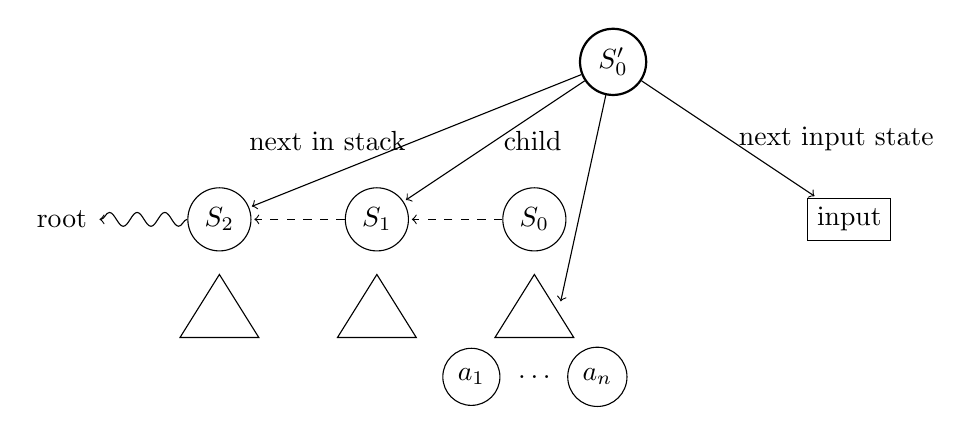
\begin{tikzpicture}[shorten >=1pt,->]
\node at (0,0) (root) {root};
\node[circle,draw] at (2,0) (c) {$S_2$};
\node[circle,draw] at (4,0) (b) {$S_1$};
\node[circle,draw] at (6,0) (top) {$S_0$};
\node[draw] at (10,0) (input) {input};
\node[circle,draw,thick] at (7,2) (new) {$S_0'$};
\node[circle,draw] at (5.2,-2) (top1) {$a_1$};
\node[circle,draw] at (6.8,-2) (topn) {$a_n$};
\node[] at (6,-2) (dots) {$\dots$};
\node[] at (6.3,-1.2) (children) {};
\draw[snake=snake] (c) -- (root);
\draw[dashed] (top) -- (b);
\draw[dashed] (b) -- (c);
\draw[sharp corners] (6,-0.7) -- (6.5,-1.5) -- (5.5,-1.5) -- cycle;
\draw[sharp corners] (4,-0.7) -- (4.5,-1.5) -- (3.5,-1.5) -- cycle;
\draw[sharp corners] (2,-0.7) -- (2.5,-1.5) -- (1.5,-1.5) -- cycle;
\draw (new) -- node [anchor=west] {child} (b);
\draw (new) -- node [anchor=east] {next in stack} (c);
\draw (new) -- node [anchor=west] {next input state} (input);
\draw (new) -- (children);
\end{tikzpicture}

\section{Left Arc}

Precondition: stack contains two subsequent nodes

Given a stack ending in $S_0$, create an arc between $S_0$ and $S_1$ so that $S_0$ is a child of $S_1$.
\begin{itemize}
\item Clone $S_1$ as $S_1'$, including its children list ($a_1 \dots a_n$).
\item Add $S_0$ to the children of $S_1'$.
\item Link back $S_1'$ to $S_2$ in the stack.
\item Link $S_1'$ to next input state (same as in $S_0$).
\item Push to list of {\it open} without modifying the context.
\end{itemize}

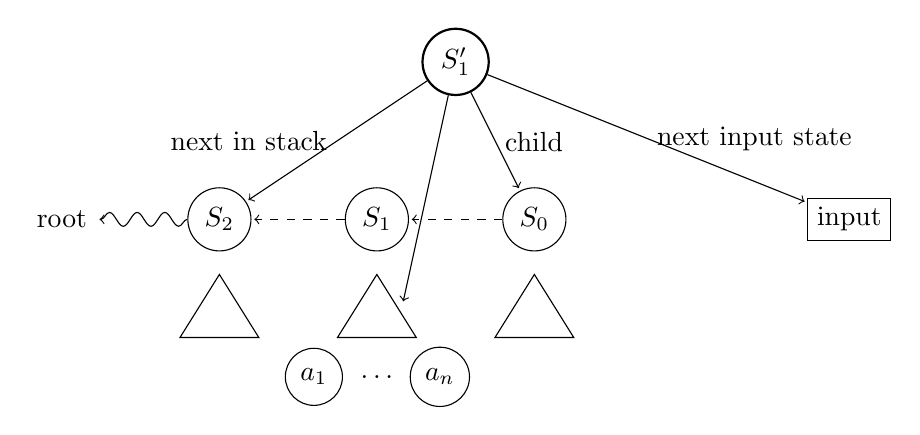
\begin{tikzpicture}[shorten >=1pt,->]
\node at (0,0) (root) {root};
\node[circle,draw] at (2,0) (c) {$S_2$};
\node[circle,draw] at (4,0) (b) {$S_1$};
\node[circle,draw] at (6,0) (top) {$S_0$};
\node[draw] at (10,0) (input) {input};
\node[circle,draw,thick] at (5,2) (new) {$S_1'$};
\node[circle,draw] at (3.2,-2) (top1) {$a_1$};
\node[circle,draw] at (4.8,-2) (topn) {$a_n$};
\node[] at (4,-2) (dots) {$\dots$};
\node[] at (4.3,-1.2) (children) {};
\draw[snake=snake] (c) -- (root);
\draw[dashed] (top) -- (b);
\draw[dashed] (b) -- (c);
\draw[sharp corners] (6,-0.7) -- (6.5,-1.5) -- (5.5,-1.5) -- cycle;
\draw[sharp corners] (4,-0.7) -- (4.5,-1.5) -- (3.5,-1.5) -- cycle;
\draw[sharp corners] (2,-0.7) -- (2.5,-1.5) -- (1.5,-1.5) -- cycle;
\draw (new) -- node [anchor=west] {child} (top);
\draw (new) -- node [anchor=east] {next in stack} (c);
\draw (new) -- node [anchor=west] {next input state} (input);
\draw (new) -- (children);
%\draw (new) -- (top1);
%\draw (new) -- (topn);
\end{tikzpicture}

\end{document}
